%Multiuser Precoding for synchronous CDMA. This presentation scheduled on Nov. 21st, 2002

\documentclass[20pt,landscape]{foils}
\usepackage[pdftex]{color}
\usepackage[pdftex]{graphicx}
\usepackage[pdftex]{geometry}
\geometry{headsep=2ex,hscale=0.9} \pdfpagewidth=11in
\pdfpageheight=8.5in

\setlength{\footskip}{0.0in} \setlength{\textheight}{8.0in}

\usepackage{background}
\usepackage{pp4slide}
%\usepackage{pdfscreen}

\newcommand{\br}{{\mathbf r}}
\newcommand{\bA}{{\mathbf A}}
\newcommand{\ba}{{\bf a}}
\newcommand{\bb}{{\bf b}}
\newcommand{\bc}{{\bf c}}
\newcommand{\bC}{{\bf C}}
\newcommand{\bd}{{\bf d}}
\newcommand{\be}{{\bf e}}
\newcommand{\bh}{{\bf h}}
\newcommand{\bbm}{{\bf m}}
\newcommand{\bt}{{\bf t}}
\newcommand{\bs}{{\bf s}}
\newcommand{\bn}{{\bf n}}
\newcommand{\bu}{{\bf u}}
\newcommand{\bv}{{\bf v}}
\newcommand{\bw}{{\bf w}}
\newcommand{\bx}{{\bf x}}
\newcommand{\by}{{\bf y}}
\newcommand{\bbf}{{\bf f}}
\newcommand{\bF}{{\bf F}}
\newcommand{\bH}{{\bf H}}
\newcommand{\bL}{{\bf L}}
\newcommand{\bM}{{\bf M}}
\newcommand{\bN}{{\bf N}}
\newcommand{\bbP}{{\bf P}}
\newcommand{\bQ}{{\bf Q}}
\newcommand{\bS}{{\bf S}}
\newcommand{\bT}{{\bf T}}
\newcommand{\bD}{{\bf D}}
\newcommand{\bX}{{\bf X}}
\newcommand{\bY}{{\bf Y}}
\newcommand{\bP}{{\bf P}}
\newcommand{\bI}{{\bf I}}
\newcommand{\bR}{{\bf R}}
\newcommand{\bU}{{\bf U}}
\newcommand{\bV}{{\bf V}}
\newcommand{\bW}{{\bf W}}
\newcommand{\bJ}{{\bf J}}
\newcommand{\bB}{{\bf B}}
\newcommand{\bzero}{{\bf 0}}
\newcommand{\bgamma}{{\mbox {\boldmath $\gamma$}}}
\newcommand{\btheta}{{\mbox {\boldmath $\theta$}}}
\newcommand{\bLambda}{{\mbox {\boldmath $\Lambda$}}}
\newcommand{\bPsi}{{\mbox {\boldmath $\Psi$}}}
\newcommand{\bPhi}{{\mbox {\boldmath $\Phi$}}}
\newcommand{\bcS}{{\mbox {\boldmath ${\cal S}$}}}
\newcommand{\bcH}{{\mbox {\boldmath ${\cal H}$}}}
\newcommand{\bcI}{{\mbox {\boldmath ${\cal I}$}}}
\newcommand{\bcP}{{\mbox {\boldmath ${\cal P}$}}}
\newcommand{\bcQ}{{\mbox {\boldmath ${\cal Q}$}}}
\newcommand{\bcR}{{\mbox {\boldmath ${\cal R}$}}}
\newcommand{\bcB}{{\mbox {\boldmath ${\cal B}$}}}

\zerolistvertdimens

\begin{document}
\raggedright \color{black}
\definecolor{bgcolor}{rgb}{1,1,1}
\pagecolor{bgcolor} % set background color
\definecolor{bgblue}{rgb}{0.04,0.37,0.59}
\vpagecolor{bgblue}


\foilhead{\LARGE Transmitter Multiuser Precoding for Synchronous
CDMA Systems}

\begin{center}
\vspace{.3in}
{\bf Shu Wang \& James Jr. Caffery}  \\
{\it \vspace{0.9in} Wireless System Research Laboratory \\
\vspace{0.2in} Dept. of Elec. \& Comp. Engin. \& Comp. Scien.
\\ University of Cincinnati}
\end{center}

\foilhead{} \vspace{2.0in}
\center{\Large Introduction}



%%
\foilhead{Multiple Access Interference}
\begin{itemize}
\item In TDMA systems (GSM and IS136), MAI comes from overlapping
slots originating in other cells and from users in the same cell
due to channel dispersion.

\item In orthogonal CDMA systems (IS95, CDMA2000 and WCDMA), the
orthogonality can not be guaranteed at each receiver once they go
through the channel. Especially in asynchronous case. MAI is hard
to be avoided even in the absence of channel distortion or
other-cell interference.

\item In FDMA systems (AMPS), extra guard bands have to be used to
separate different users.

\item In some other MIMO system, such as OFDM and DMT, MAI can
appear as ISI or cross talk.
\end{itemize}


%%
\foilhead{Emerging Mitigation Technologies}
\begin{itemize}
\item Transmitter Design

    \begin{itemize}
     \item Multiuser precoding: optimal (nolinear) and linear.
     \item Transmitter diversity. selective transmission and advanced channel
     coding.
    \end{itemize}

\item Receiver Detection

    \begin{itemize}
     \item Multiuser detection: optimal, linear and nolinear.
     \item Receiver diversity (smart antenna): switch beamform, adaptive beamform.
    \end{itemize}


\item Tansceiver Design (system level)
    \begin{itemize}
     \item Power control: fast, open-loop and closed-loop.
     \item Sequence design (generalized orthogonal sequences): ZCZ sequences, LCZ sequences.
    \end{itemize}
\end{itemize}


%%
\foilhead{Uplink/Downlink of Synchronous CDMA System}
\begin{itemize}
\item Uplink of CDMA system

    \begin{itemize}
     \item MS: Limited computation capacity and power
     supply. Perfectly synchronized transmission can not be
     guarantee. Almost no knowledge of other active users.
     \item BS: Enough computation capacity and power
     supply in most cases. Complex receiver signal precessing can be affordable.
    \end{itemize}


\item Downlink of CDMA system

    \begin{itemize}
     \item BS: Nearly know everything about each active user in
     its cell. The signals for each user are synchronously
     transmitted.
     \item MS: Complex signal precessing for receiver usually can not be used.
    \end{itemize}

\end{itemize}


\foilhead{Basic Synchronous CDMA System Models}
\begin{figure}
\begin{center}
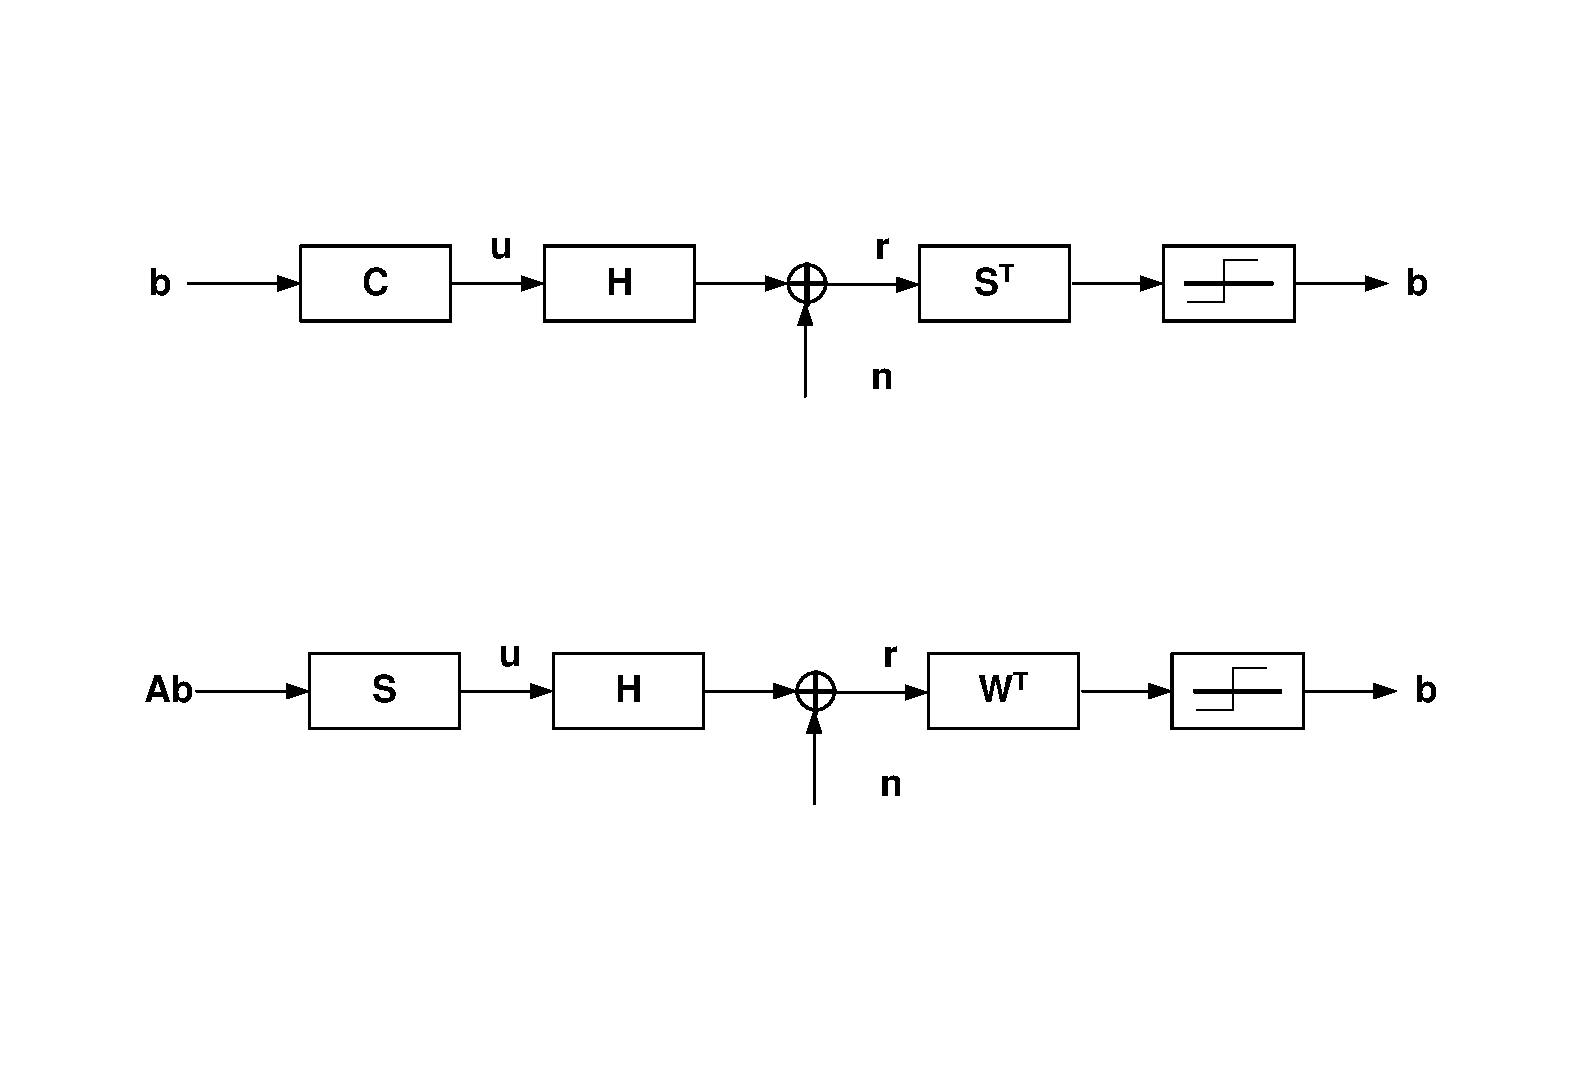
\includegraphics[width=7.0in]{SystemModels.pdf}
\end{center}
\end{figure}
\center{Classic K-user system models for multiuser precoding and
multiuser detection.}


%%
\foilhead{Transmitter Multiuser Precoding I}
\begin{itemize}
\item Compared with multiuser detection at receiver, multiuser
precoding refers to data detection in non-orthogonal multiplexes
with optimizing transmitter design,

\item The transmitter has usually known much prior information
about all the active users, such as power spectrum and symbol
shaping, in multiuser precoding.

\item The correlations among different sub-channels may be
utilized to enhance the transmission for each user in multiuser
precoding. (Multiple Access Enhancement)

\item It is much difficult for transmitter(s) to the obtain
channel information, such as channel distortion and multipath
delay, except with the help of receivers in reserve links.
\end{itemize}


\foilhead{Transmitter Multiuser Precoding II}
\begin{itemize}

\item It can alleviate the signal processing burden at receivers,
especially where the mobile stations have no enough power supply
and computation capacity.

\item With multiuser precoding, the non-orthogonal spreading
sequences may be used without receiver multiuser detection.
Therefore, it can increase the number of sustainable users in
system as multiuser detection does.

\item If channel information is available, it can compensate
channel distortion at transmitters as Tomlinson pre-equalization.

\item It can also reduce the reliance on tight and accurate power
control. In some cases, we can even utilize the correlations among
different spreading sequences to enhance the transmission for
desired users.
\end{itemize}


\foilhead{Classification of Transmitter Multiuser Precoding}
\begin{itemize}
\item Most concepts in multiuser receiver design can also be
applied for transmitter multiuser precoding.

\item Nonlinear/optimal multiuser precoding:
    \begin{itemize}
    \item individually optimum multiuser precoding.
    \item jointly optimum multiuser precoding.
    \end{itemize}
\item Linear multiuser precoding:
    \begin{itemize}
    \item decorrelating multiuser precoding.
    \item minimum mean squares error (MMSE) multiuser precodings.
    \item maximum asymptotic multiuser efficiency (MAME) multiuser precoding.
    \item approximated maximum likelihood (AML) multiuser precoding.
    \end{itemize}
\end{itemize}


%%
\foilhead{Other Related Techniques}
\begin{itemize}
\item Tomlinson pre-equalization (M. Tomlinson, 1971). With moving
receiver equalization up to transmitter design, receiver design
may be greatly simplified.

\item Spreading sequence design for CDMA (N. Suehiro, 1994). With
exploring the algebraic properties of binary, quadriphase and
non-binary sequences, the spreading sequence can be designed to be
resistant to the multipath interferences of small delays.

\item Convolutional FEC coding (P. Elias, 1955) and block channel
coding (T. Liew and L. Hanzo, 2002). With adding redundancy and
using special combination, the coded input bit stream has more
resistance to channel distortion and interference.
\end{itemize}


\foilhead{}
\vspace{2.0in}{\Large Optimum Multiuser Precoding}

%%
\foilhead{Optimum Multiuser Precoding}

\begin{itemize}
 \item In optimum multiuser precoding, all the users' BER are minimized with some criterium.
 \item Optimum multiuser precoding is decided not only by spreading sequences and SNRs but also by input vector and transmission power distribution for
 each user.
 \item The definitions of individually optimum multiuser precoding and
 detection may be different.
 \item The channel matrix $\bH$ is to be $\bI$ in optimum
 multiuser precoding.
\end{itemize}


%%
\foilhead{Jointly Optimum Multiuser Precoding I}
\begin{itemize}
\item Jointly optimum multiuser precoding $\bC_{JP}$ is design to
minimize the errors in output bit vectors.

$$\matrix{\bC_{JP}&=&\min\limits_{\bC}P[\hat\bb\neq\bb]}$$

\item Decision regions.  The decision region for user $k$ is given
by

$$\matrix{\hat{b}_k&=&\min\limits_{\bar{b}_k}\|\bC\bb+\bn-\bar{b}_k\bs_k\|}$$

\item Bit-error rate.

$$
\begin{array}{rcl}
P_e&=&1-{1\over(2\pi\sigma^2)^{L/2}}\mbox{E}\left\{\int_{\bcR(\bb)}e^{-{1\over2\sigma^2}\left\|\bx-\bC\bb\right\|_2^2}\mbox{d\bx}\right\}
\end{array}
$$
\end{itemize}


%%
\foilhead{Jointly Optimum Multiuser Precoding II}
\begin{itemize}

\item the jointly optimum precoder $\bC_{JP}$ can be expressed as

$$
\begin{array}{rcl}
\bC_{JP}&=&\bar{\bS}\bA
\end{array}
$$

\noindent where $\bar{\bS}=[b_1\bar\bs\ b_2\bar\bs\ \ldots
b_K\bar\bs]$ and $\bar{\bs}=\|\bS\bb\|_2^{-1}\bS\bb$

\item Actually, all the user share the same spreading sequence
$\bar{\bs}$.

\item Different input $\bb$ and amplitude distribution $\bA$ lead
to different optimum precoder $\bC_{JP}$ and spreading sequence
$\bar{\bs}$.

\end{itemize}


\foilhead{Example: Decision Regions For A 2-User Case}
\begin{figure}
\begin{center}
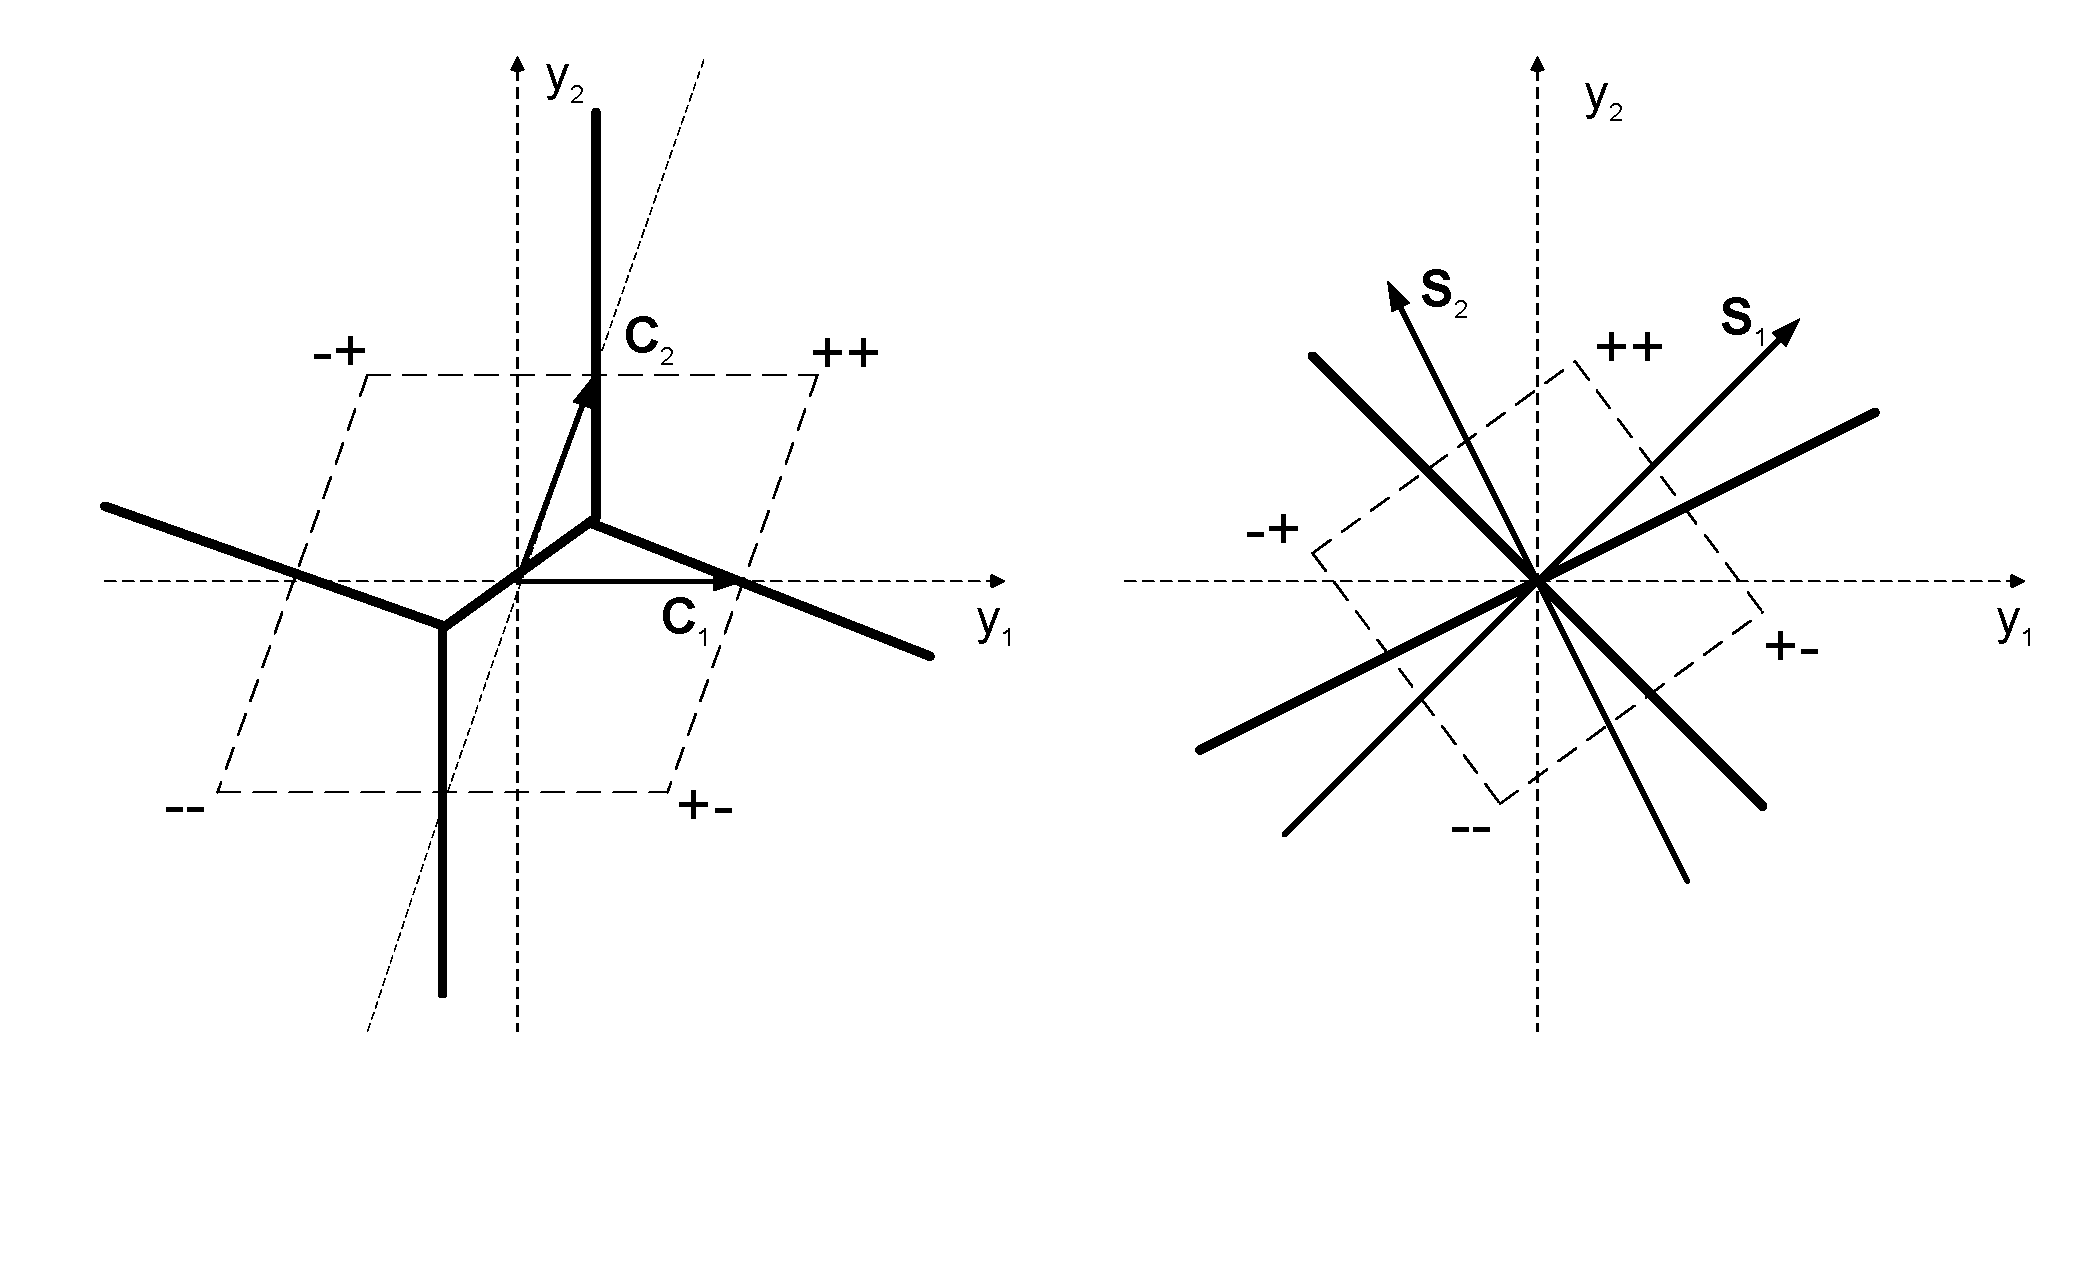
\includegraphics[width=8.0in]{JP_DecisionRegs.pdf}
\end{center}
\end{figure}



\foilhead{Example: Signal Space Demonstration for A 2-User Case}
\begin{figure}
\begin{center}
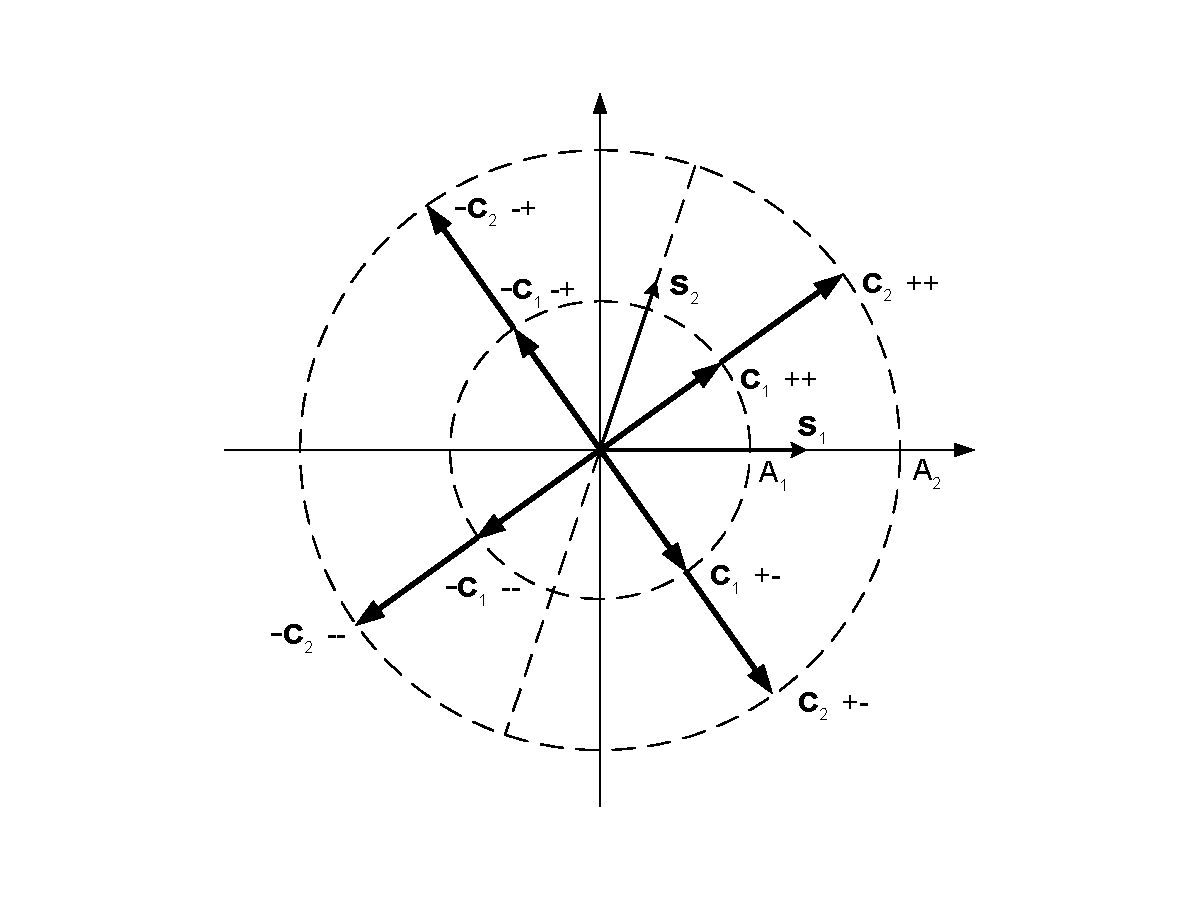
\includegraphics[width=7.0in]{JP.pdf}
\end{center}
\end{figure}

%%
\foilhead{Individually Multiuser Precoding}
\begin{itemize}
\item Different to individually optimum multiuser detection, the
individually optimum multiuser precoding $\bC_{IP}$ is given by

$$
\begin{array}{rcccl}
\bC_{IP}&=&\mbox{arg}\min\limits_{\bC}\prod\limits_{k=1}^{K}(P_{ek})^{w_k}&=&\mbox{arg}\min\limits_{\bC}\prod\limits_{k=1}^{K}\left\{\mbox{E}\left[Q\left({\bs_k^T\bC\bd_k\over\sigma}\right)\right]\right\}^{w_k}
\end{array}\label{individually4}
$$

\item The $w_k$ is introduced to separate BER performances for
different users.

\item Due to the absolution functions and integral functions in
the definition, it is hard to give a close-form solution here.

\end{itemize}

%%
\foilhead{Example: 2-User Individu. Optimum Multiuser Precoding I}

Example: Suppose that there are only two users with $A_2=2A_1$ and
$\rho=1/3$. The 2nd user's weight $w_2$ is set to be $4$.

\vspace{0.50in}Numerical Solution: The individually optimum
precoding can be searched out and expressed is

\begin{itemize}
\item when $b_1=b_2$

$$
\bC_{IP}\approx[\matrix{A_1(0.7089\bs_1+0.7053\bs_2)&A_2(0.1724\bs_1+0.9850\bs_2)}]
$$

\item When $b_1=-b_2$

$$
\bC_{IP}\approx[\matrix{A_1(0.7071\bs_1-0.7071\bs_2)&A_2(\mbox{-0.0698}\bs_1+0.9976\bs_2)}]
$$

\end{itemize}

\foilhead{Example: 2-User Individu. Optimum Multiuser Precoding II
II}
\begin{figure}
\begin{center}
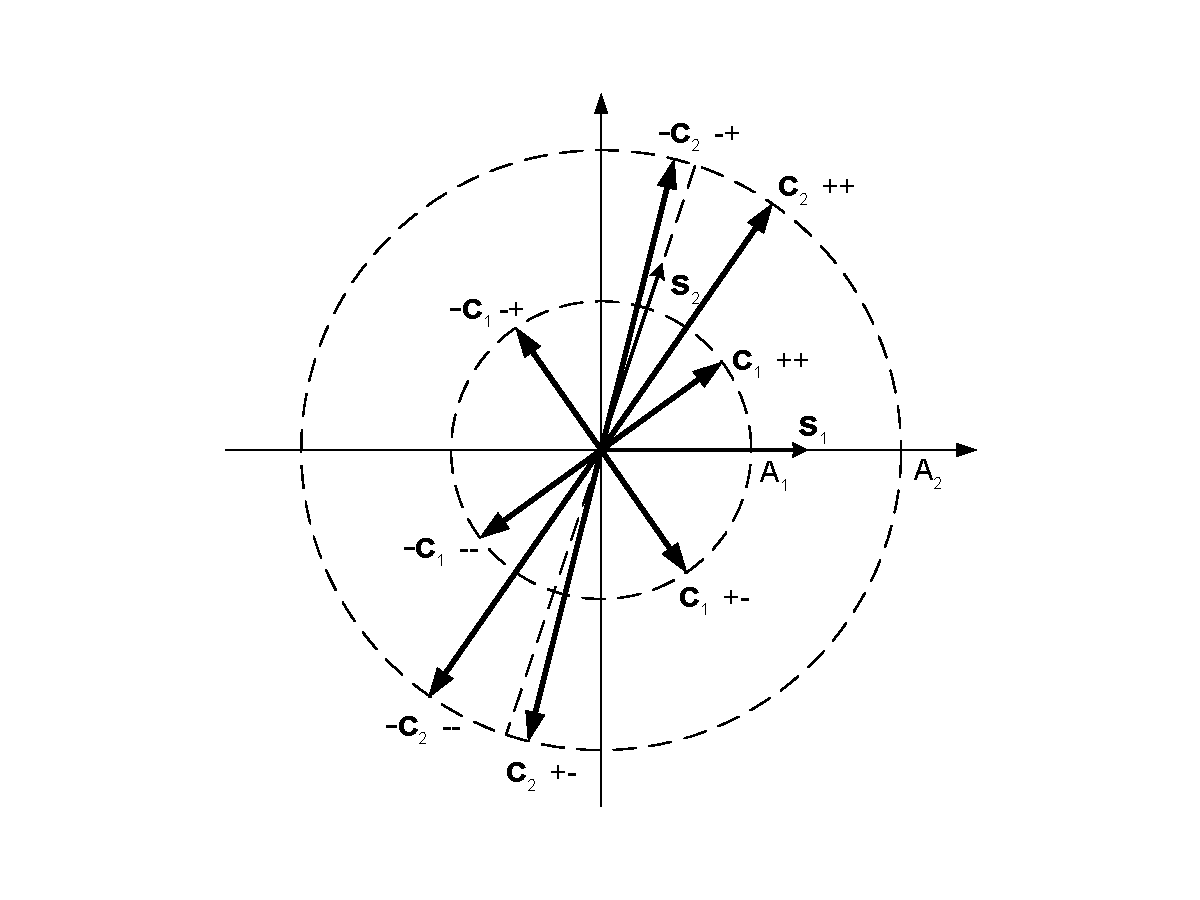
\includegraphics[width=7.0in]{IP_example.pdf}
\end{center}
\end{figure}


\foilhead{Computer Simulations I}
\begin{figure}
\begin{center}
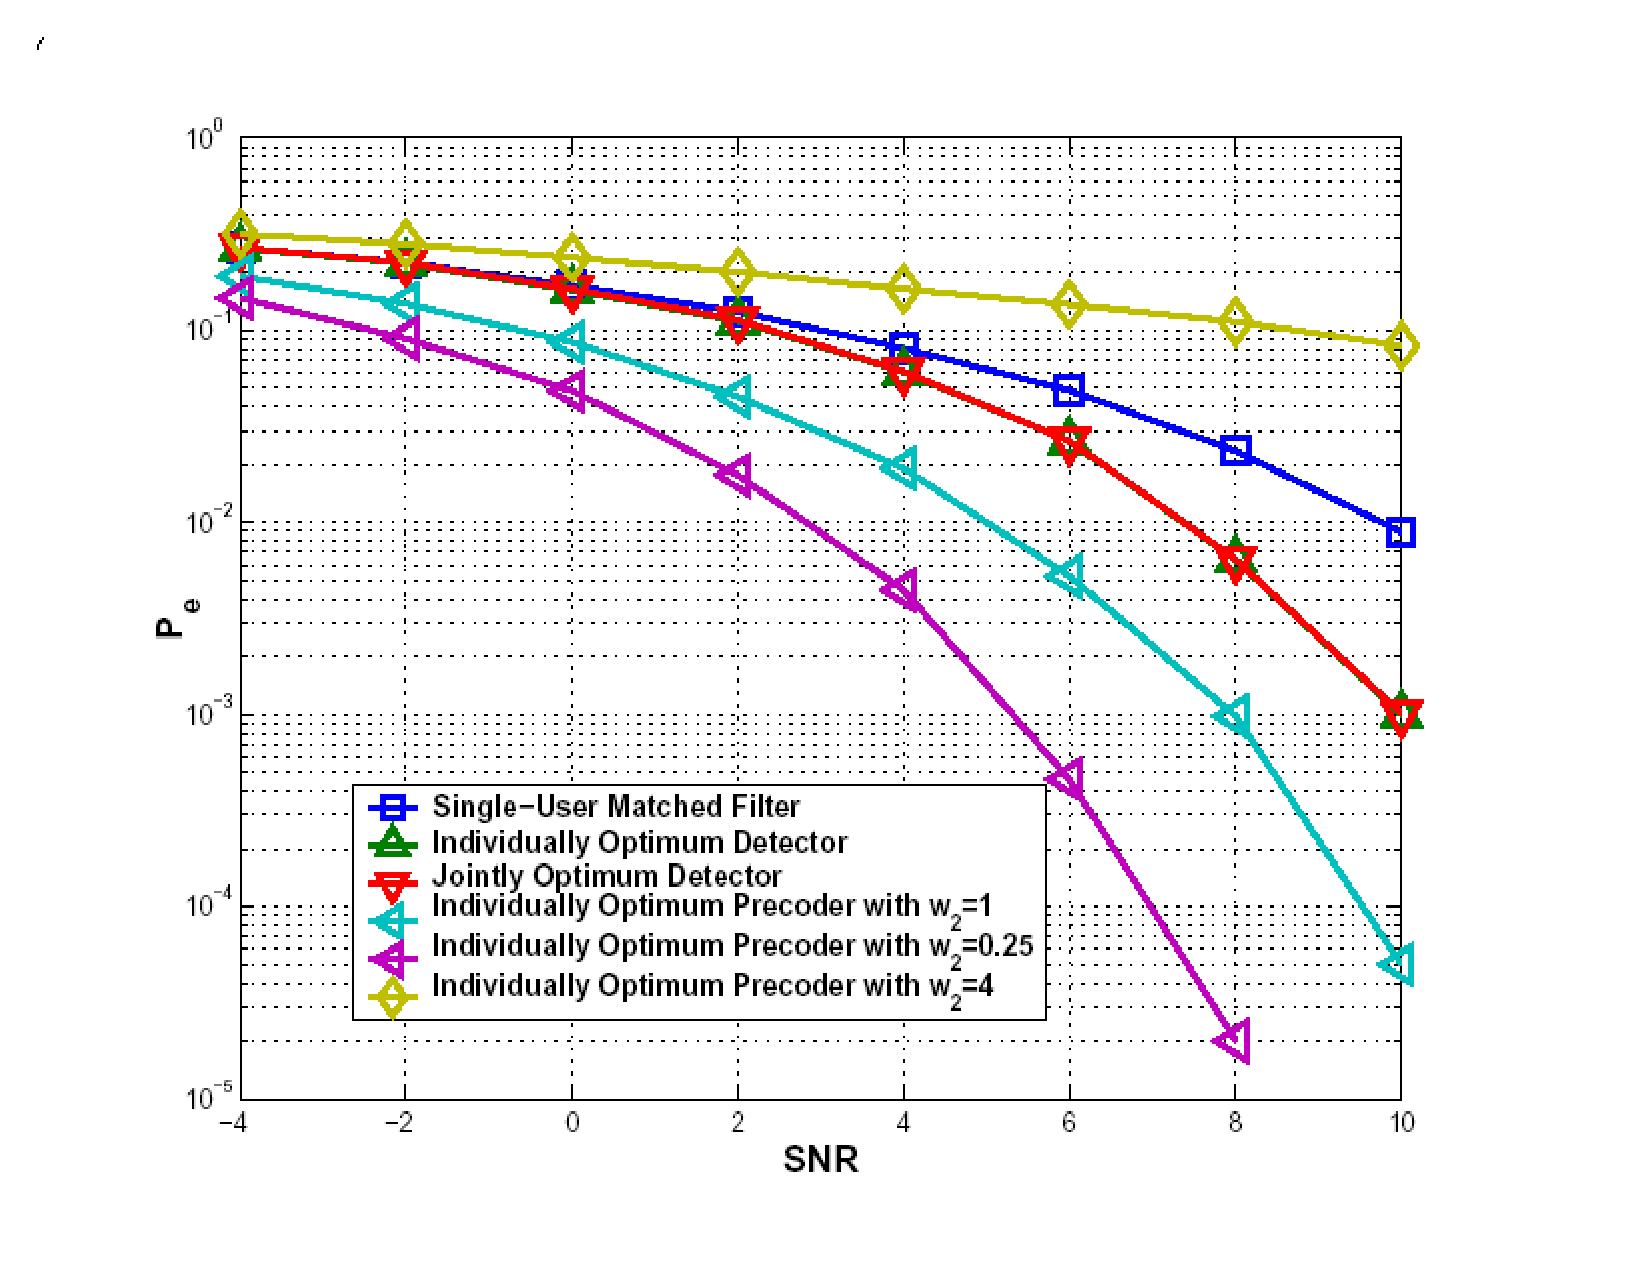
\includegraphics[width=8.0in]{Opt_BER.pdf}
\end{center}
\end{figure}


\foilhead{Computer Simulations II}
\begin{figure}
\begin{center}
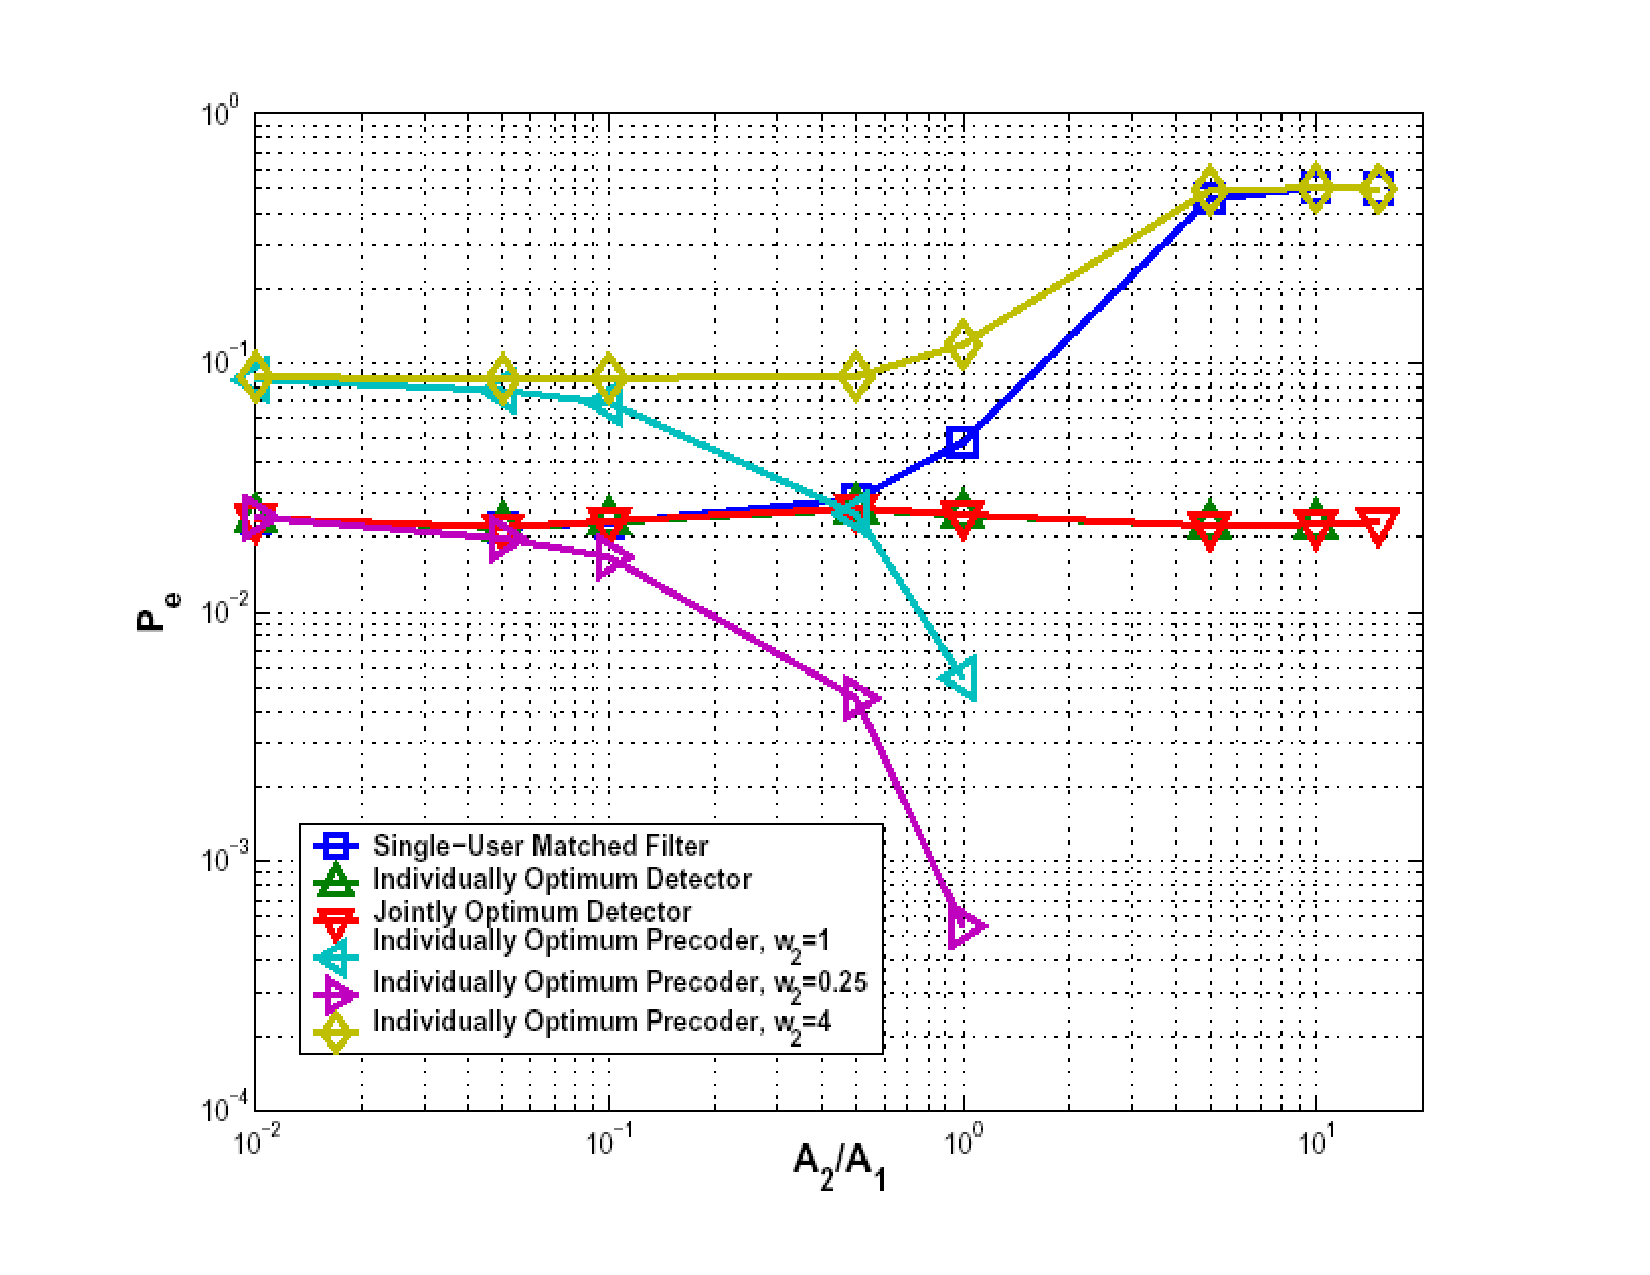
\includegraphics[width=8.0in]{Opt_NFR.pdf}
\end{center}
\end{figure}


\foilhead{}

\vspace{2.0in}{\Large Linear Multiuser Precoding}

%%
\foilhead{Linear Multiuser Precoding}
\begin{itemize}
\item The linear precoding $\bC$ is independent to input bit
vector $\bb$.

\item Most of linear multiuser receiver optimization schemes are
applicable here:
    \begin{itemize}
    \item minimizing multiple access interference. (decorrelating multiuser precoding)
    \item minimizing mean squares error. (MMSE multiuser precoding)
    \item maximizing likelihood function. (ML or approximated ML multiuser precoding)
    \item maximizing asymptotic multiuser efficiency. (MAME multiuser precoding)
    \end{itemize}
\item In most cases, additional constrains should be considered:
    \begin{itemize}
    \item total power constraint. $\sum A_k^2=P$ is fixed.
    \item power spectrum constraint. $A_k$ is fixed.
    \item maximum eigenvector constraint.
    $P_t = \left\|\bC\bb\right\|_2^2\leq K\|\bC\|_2^2 = K\lambda_{\max}\left(\bC\bC^T\right)$
    \end{itemize}
\end{itemize}



%%
\foilhead{Decorrelating Multiuser Precoding}
\begin{itemize}
\item Decorrelating precoding can be expressed as in the following
optimization problem.

$$\begin{array}{rcl}
\bC_{DP}&=&\mbox{arg}\min\limits_{\bC}\left\|\bS^T(\bH\bC\bb-\bn)-\bA\bb\right\|_2\hspace{0.1in},
\end{array}\label{DD}$$

\item The least-square (LS) solution to the above unconstrained
optimization problem can be expressed as

$$\begin{array}{rcl}
\bC_{LS}&=&(\bS^T\bH)^{+}\bA\hspace{0.1in},
\end{array}\label{C-DDLS}$$

\item No noise enhancement. This is at expense of signal
enhancement.

\end{itemize}



%%
\foilhead{MMSE Multiuser Precoding I}
\begin{itemize}
\item A common approach in signal estimation theory to the problem
of estimating a random variable $\bb$ on the basis of observation
$\br$ with given constrains to choose the linear function $\bC$
that minimizes that mean-square error (MSE):

$$\begin{array}{rcl}
\bC_{MMSE}&=&\min\limits_{\bC}\left\{\mbox{E}\left\|\bS^T(\bH\bC\bb+\bn)-\bA\bb\right\|_2\right\}\hspace{0.1in},
\end{array}\label{MSE}$$

\noindent subject to some possible constraint on $\bC$.

\item The solution to this optimization equation depends on the
constraints imposed on $\bC$.
    \begin{itemize}
    \item No constraint. It becomes an unconstraint optimization
    problem.
    \item Total power constraint. $\mbox{trace}\{\bC\bC^T\}=P_t$
    \item Maximum eigenvalue constraint. $\lambda_{\max}\{\bC\bC^T\}=\lambda_t$
    \end{itemize}
\end{itemize}

%%
\foilhead{MMSE Multiuser Precoding II}
\begin{itemize}
\item The unconstrained MMSE precoder can be easily derived as

$$
\begin{array}{rcl}
\bC_{MMSE}&=&(\bS^T\bH)^{+}\bA\hspace{0.1in}.
\end{array}\label{UMMSE}
$$

\item The MMSE optimization problem under total power constraint
can be solved by means of the Lagrange multiplier method.

$$\begin{array}{rcl}
\bC_{TP}&=&(\bH^T\bS\bS^T\bH+\lambda\bI)^{-1}\bH^T\bS\bA\hspace{0.1in}.
\end{array}$$

\item The solution to the MMSE optimization problem under maximum
eigenvalue constraint

$$\begin{array}{rcl}
\bC_{MMSE-EV}&=&\sqrt{\lambda_t}\bV
\end{array}\label{C-MMSEEV}$$

\end{itemize}

%%
\foilhead{MAME Multiuser Precoding}
\begin{itemize}
\item An asymptotic multiuser efficient vector is introduced here.

$$\begin{array}{rcl}
\mathbf{\bar{\eta}}(\bC)&=&\left[\matrix{\eta_1(\bC)&\eta_2(\bC)&\ldots&\eta_K(\bC)}\right]^T
\end{array}$$

\item Instead of only maximizing the AME of one user, the norm of
the AME vector is optimized here so that all the users' AMEs are
maximized.

$$\begin{array}{rcl}
\bC_{MAME}&=&\mbox{arg}\sum\limits_{k=1}^{K}\eta_k(\bC)
\end{array}\label{MAME1}$$

\item Due to the presence of the absolute value function in the
optimization equation, it is very hard to give a close-form
solution to these nonlinear optimization problems in the $K$-user
case, except $K=2$
\end{itemize}



%%
\foilhead{Example: 2-User MAME Multiuser Precoding I}
\begin{itemize}
\item For two-user case, MAME multiuser precoding can be written
as

$$\begin{array}{rcl}
\bC_{MAME}&=&\left\{\begin{array}{lc}
\bS\bbP&{A_2\over A_1}<|\rho|\\
\bS\bU&|\rho|\leq{A_2\over A_1}<{1\over |\rho|}\\
\bS\bQ&{1\over |\rho|}\leq{A_2\over A_1}
\end{array}\right.
\end{array}$$

\item Two-user MAME multiuser precoding actually is a mixed form
of decorrelating multiuser precoding and direct spreading. This is
similar to MAME multiuser detection for two-user case.

\item It can be shown that the AME of either user with MAME
multiuser precoding is similar to that with MAME multiuser
detection in two-user case.

\end{itemize}


\foilhead{Example: 2-User MAME Multiuser Precoding II}
\begin{figure}
\begin{center}
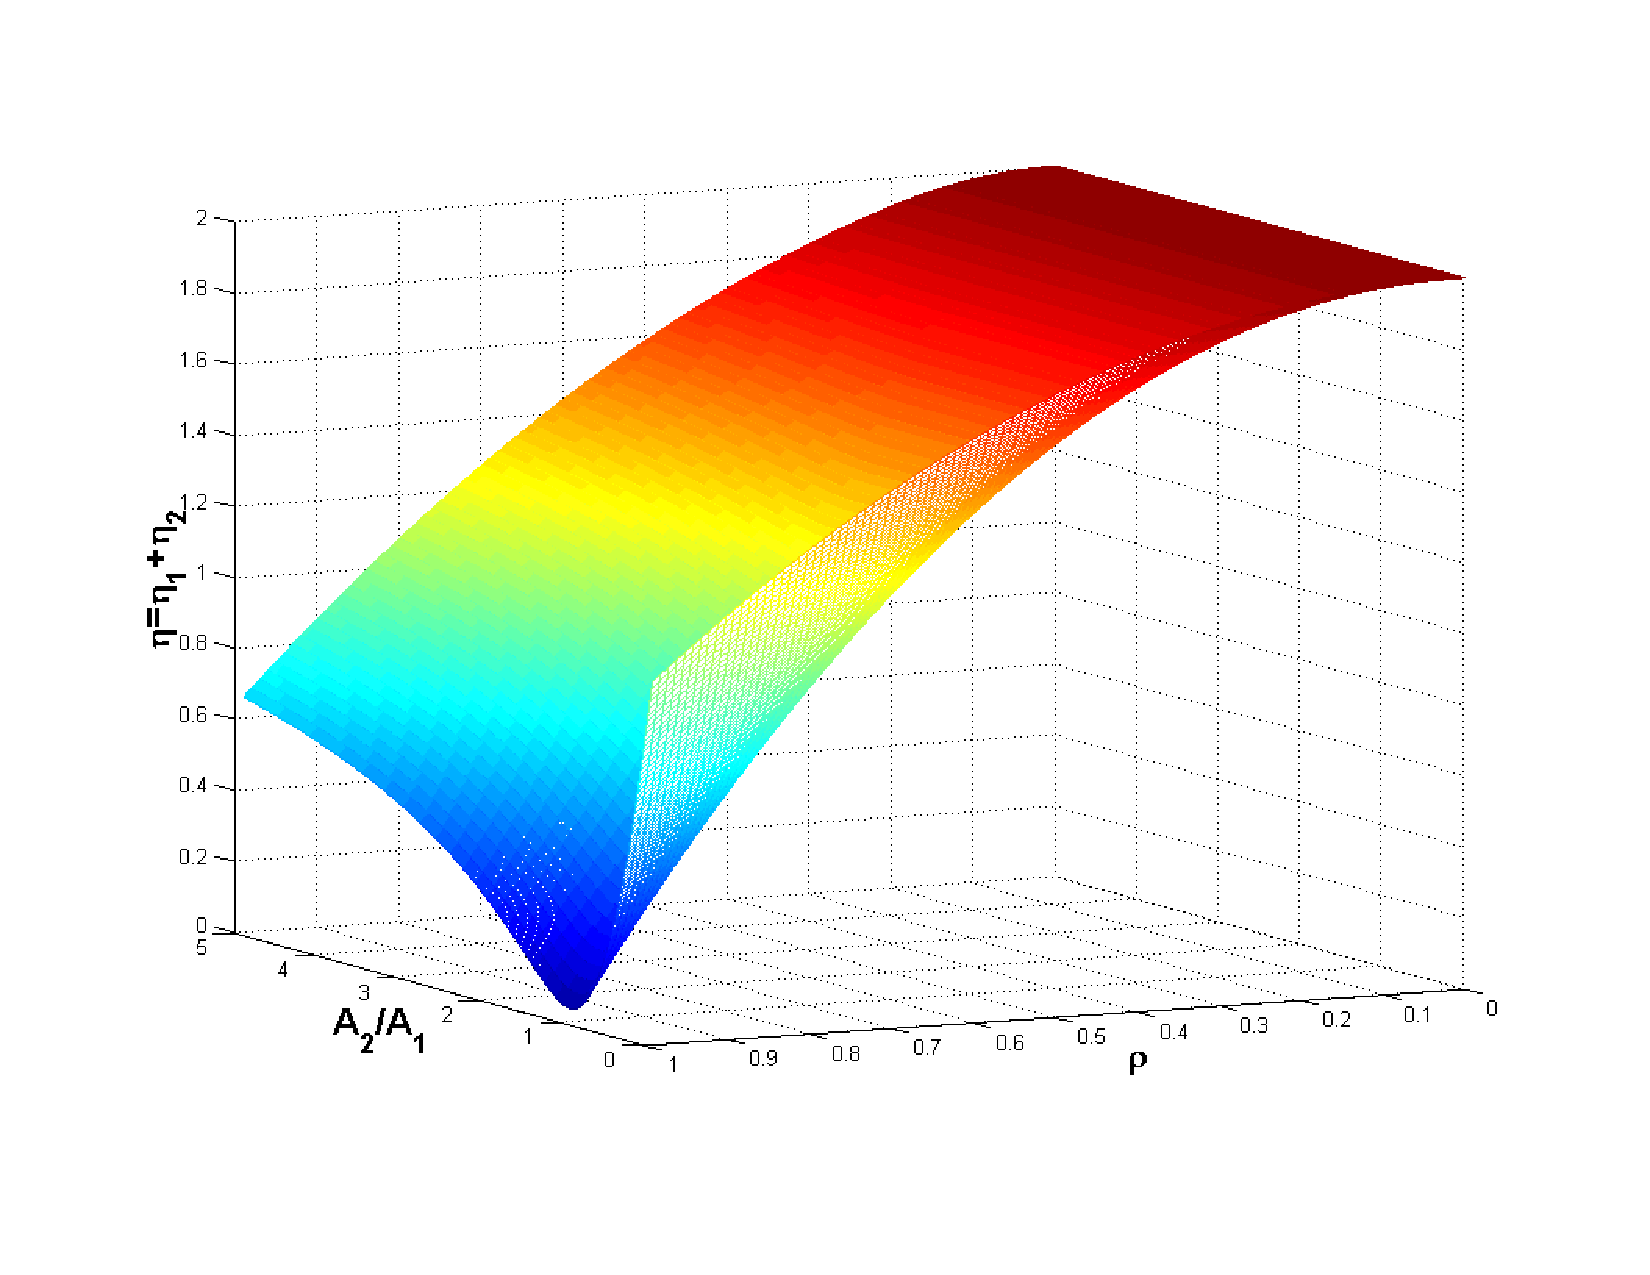
\includegraphics[width=8.0in]{AME_3D.pdf}
\end{center}
\end{figure}


\foilhead{Example: 2-User MAME Multiuser Precoding III}
\begin{figure}
\begin{center}
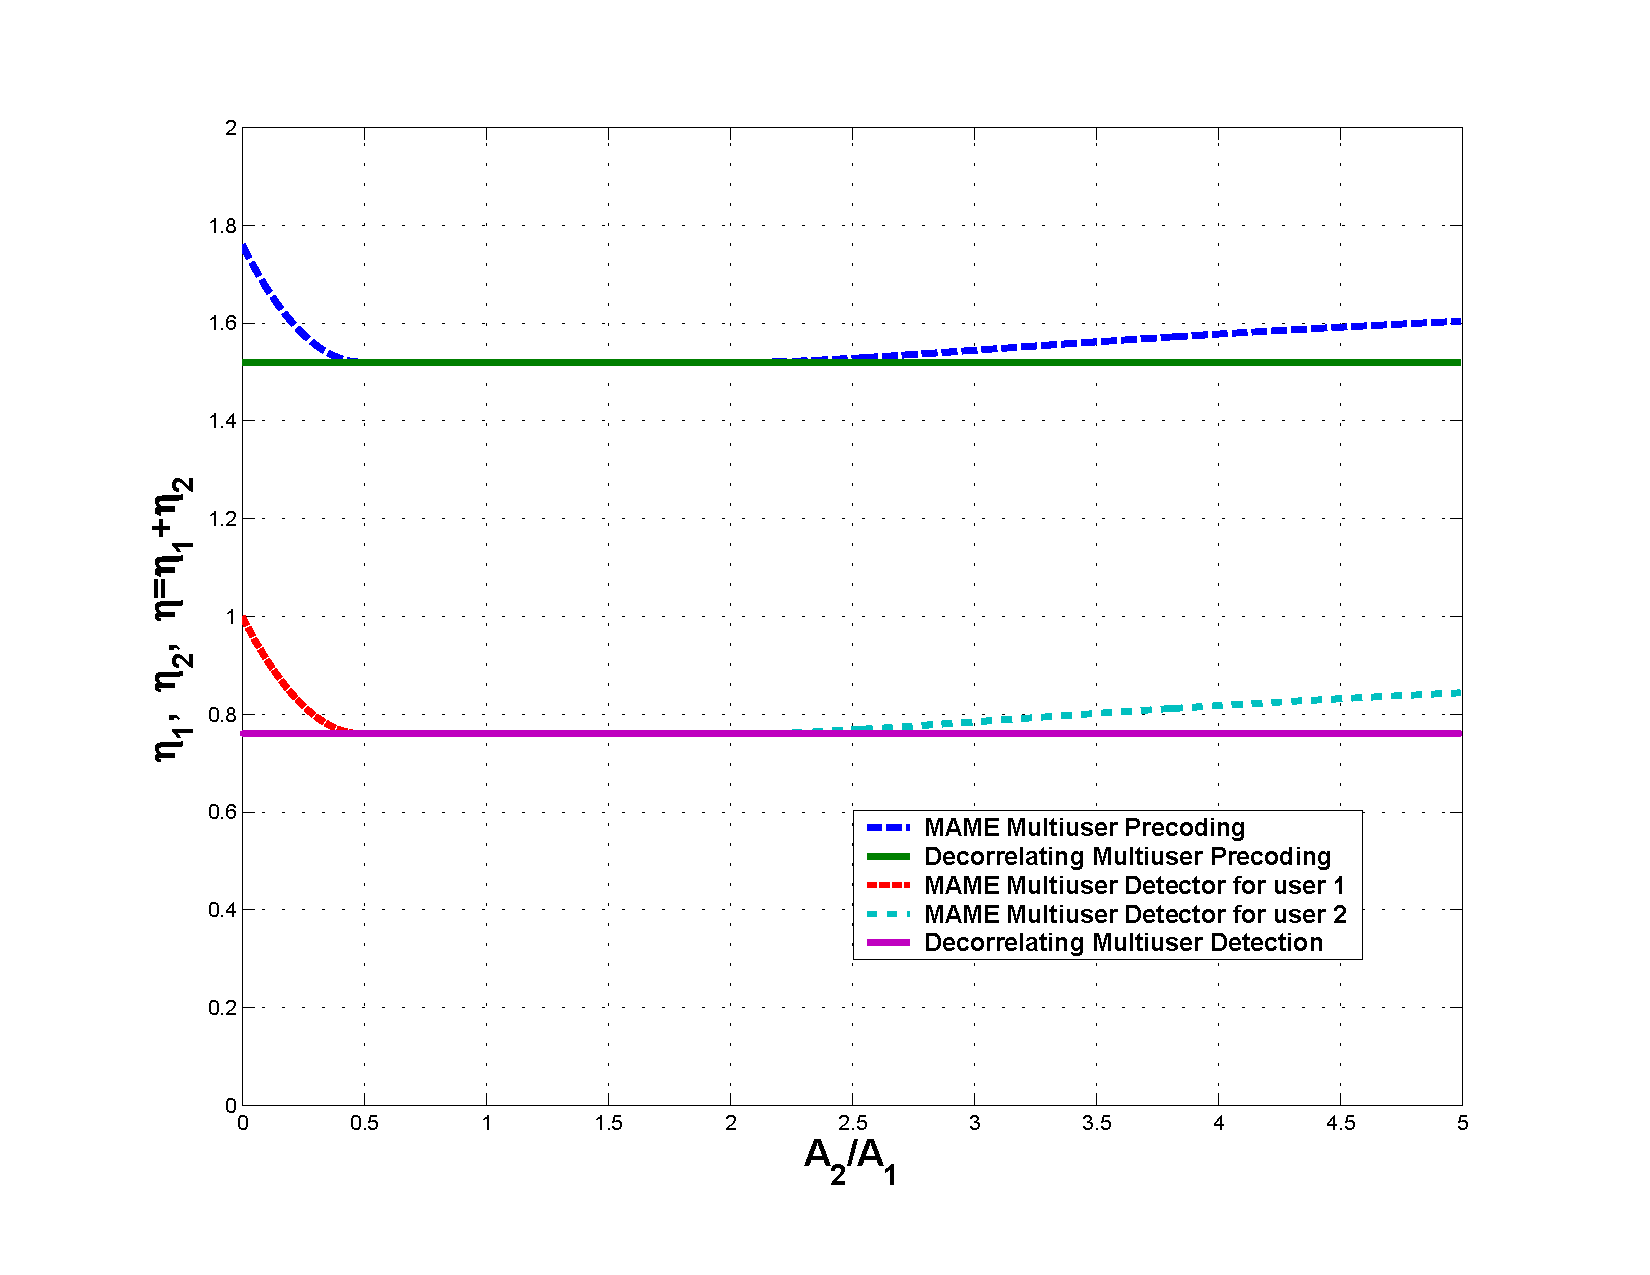
\includegraphics[width=8.0in]{AME_2D.pdf}
\end{center}
\end{figure}

%%
\foilhead{AML Multiuser Precoding I}
\begin{itemize}
\item ML transmitter optimization criterion can be expressed as in
the following maximization problem to maximize the minimum ML
distance under some possible constraint, e.g., the total
transmitting signal power constraint.
$$\begin{array}{rcl}
\bC_{ML}&=&\mbox{arg}\max\limits_{\bC}\left\{\min\limits_{k}\left[\bS^T\bH\bC\bb^k-\bA\hat{\bb}\right]^T\bR_n^{-1}\left[\bS^T\bH\bC\bb^k-\bA\hat{\bb}\right]\right\}\hspace{0.1in},
\end{array}\label{ML-P1}$$
\item The above ML precoding optimization rule can be
approximately replaced by
$$\begin{array}{rcl}
\bC_{AML}&=&\mbox{arg}\max\limits_{\bC}\left\{\lambda_{\min}(\bC^T\mathbf{\Pi}\bC)\right\}
\end{array},$$
where $\mathbf{\Pi}=\bH^T\bS\bR^{-1}\bS^T\bH$, subject to some
possible constraint on $\bC$.
\end{itemize}

\foilhead{AML Multiuser Precoding II}
\begin{itemize}
\item The solution to AML optimization under total power
constraint is given by
$$\begin{array}{rcl}
\bC_{AML-TP}&=&\bV\mathbf{\Phi}_{TP}
\end{array}\label{ML-P6}$$
where $\bV$ consists of the $K$ orthogonal eigenvectors of the
matrix $\bH^T\bS\bR^{-1}\bS^T\bH$, $\mathbf{\Phi}_{TP}$ is a
diagonal matrix with diagonal elements $\phi_{PT}^k$ and
$|\phi_{TP}^k|^2=P_t(\lambda_k\sum\limits_{i=1}^{K}\lambda_i)^{-1}$
\item The solution to AML optimization under maximum eigenvalue
constraint is given by
$$\begin{array}{rcl}
\bC_{AML-EV}&=&\bV\mathbf{\Phi}_{EV}
\end{array}\label{C-MLEV}$$
where $\mathbf{\Phi}_{EV}$ is a diagonal matrix with diagonal
elements $\phi_{EV}^k$ and
$|\phi_{EV}^k|^2={\lambda_N\over\lambda_k}\lambda_t$.

\end{itemize}


\foilhead{Computer Simulations I}
\begin{figure}
\begin{center}
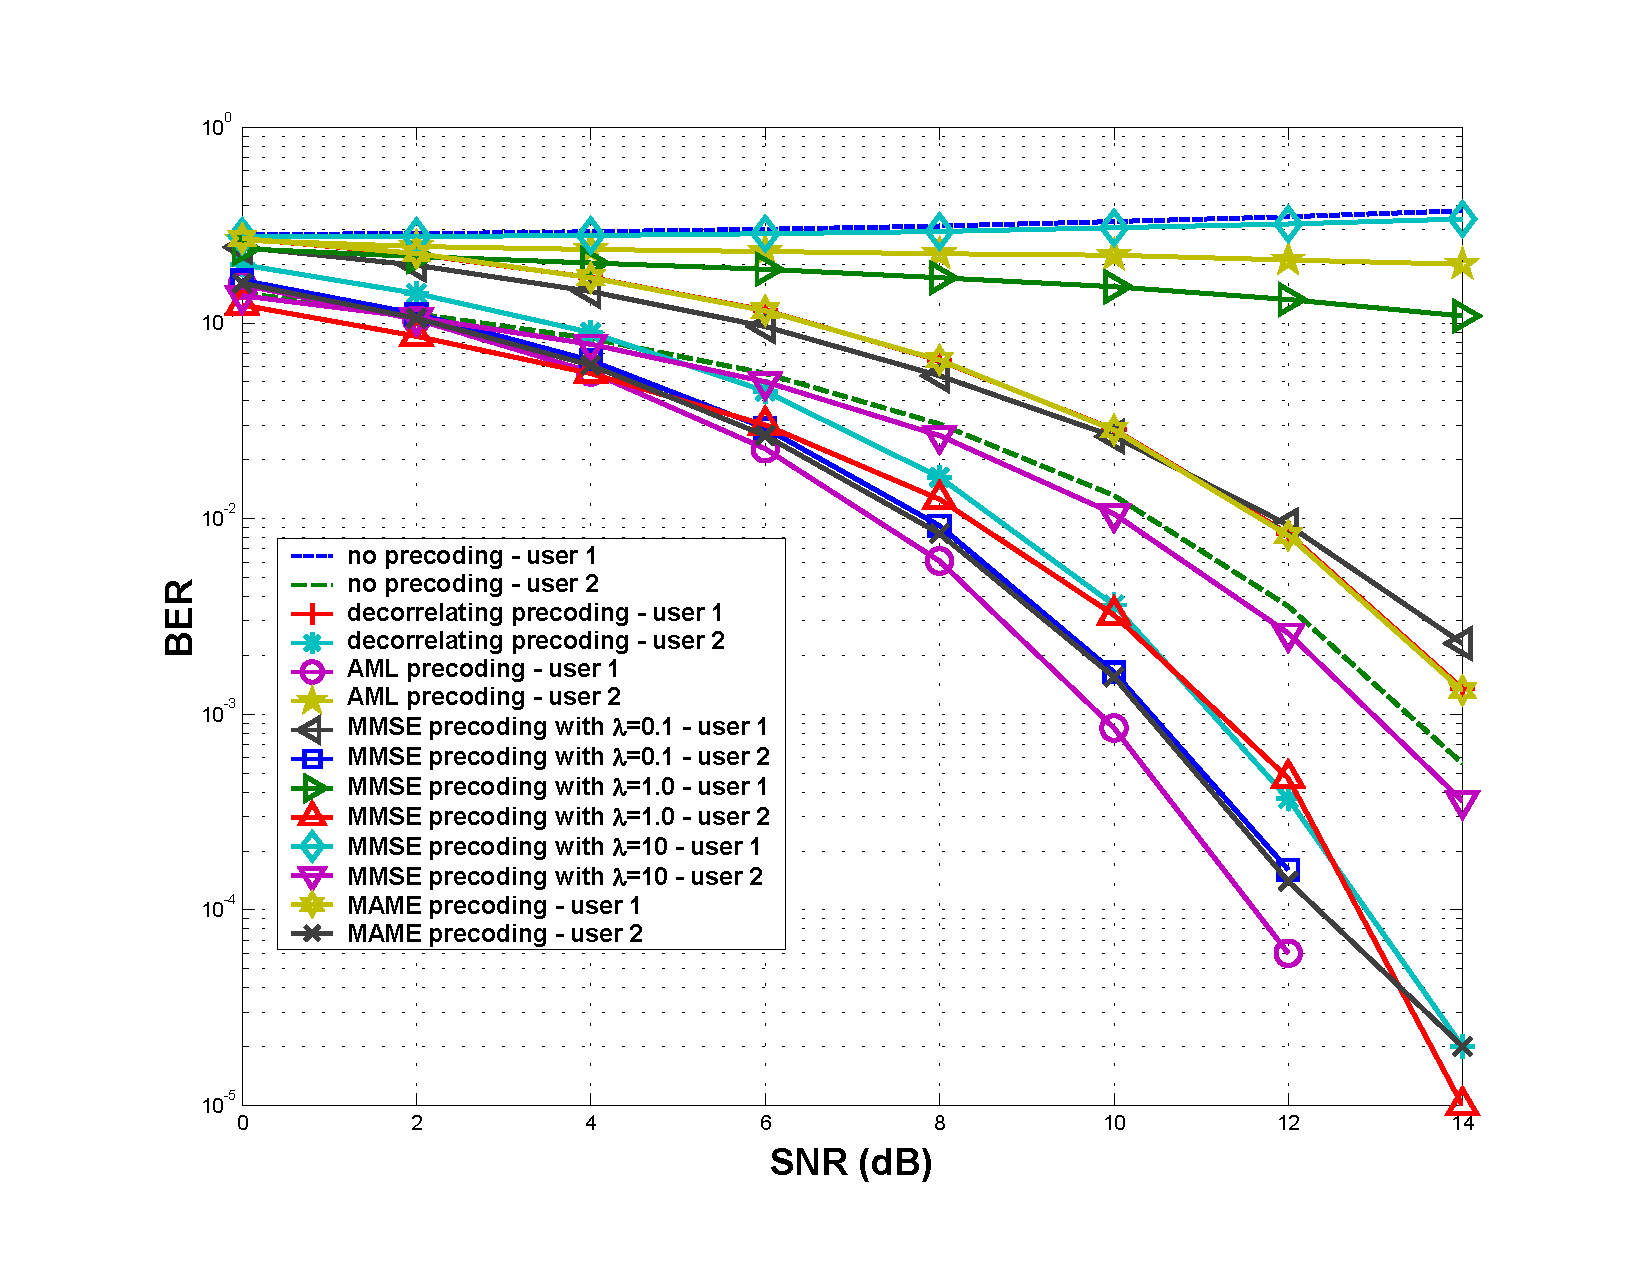
\includegraphics[width=7.0in]{Linear_BER.pdf}
\end{center}
\end{figure}


\foilhead{Computer Simulations II}
\begin{figure}
\begin{center}
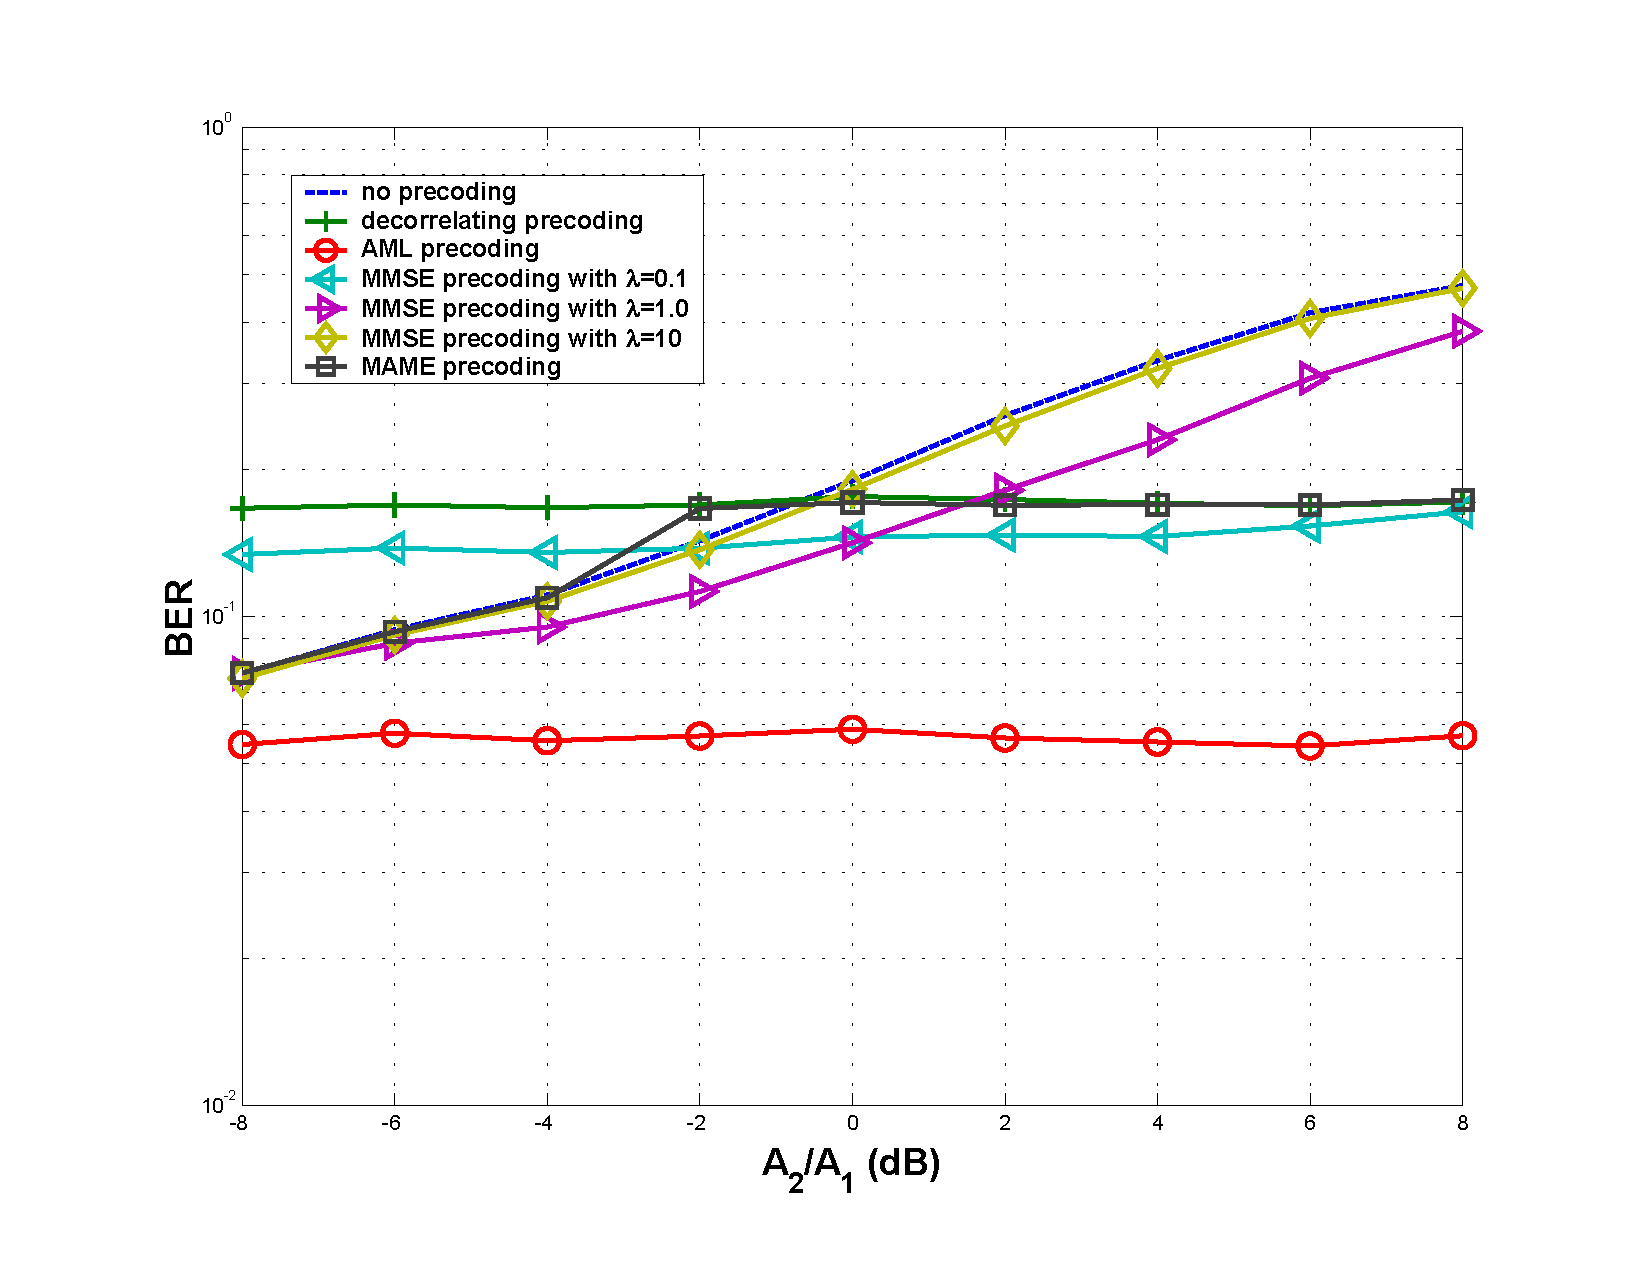
\includegraphics[width=7.0in]{Linear_NFR.pdf}
\end{center}
\end{figure}

%%
\foilhead{Conclusion \& Future Directions}
\begin{itemize}
\item With more prior user information, it is possible for optimum
multiuser precoding to achieve better performance than multiuser
detection. (Multiuser Interference Enhancement)

\item With linear system theory, it can be shown that many linear
multiuser precoders and detectors can achieve the same
performance.

\item Additional performance enhancement may be achievable by
combining transmitter multiuser precoding and adaptive
receivers/transmitters.

\item For unknown or time-variable channels, spreading sequence
adaption or adaptive multiuser precoding with feedback from
receivers can be an interesting topic.

\item For unknown or time-variable channels, multiuser precoding
can be jointly used with channel coding to achieve a better
performance.

\end{itemize}

%%
\foilhead{Selected References}
\begin{itemize}\tiny

\item M. Tomlinson, New automatic equaliser employing modulo
arithmetric, Electronics Letter, Vol. 7, pp.138-139, March 1971.

\item G. D. Forney, Jr., M.V. Eyuboglu, Combined equalization and
coding using precoding, IEEE Communications Magazine , Vol. 29
No.12 , December 1991 pp. 25-34.

\item N. Suehiro, A signal design without co-channel interference
for approximately synchronized CDMA systems, IEEE Journal on
Selected Area In Communication, No. 5, Vol. 12, pp. 837-841, June
1994.

\item Pingzhi Fan and Li Hao, Generalized orthogonal sequences and
their applications in synchronous CDMA systems. IEICE Transactions
On Fundamentals, E83-A(11): 2054-2069, November 2000.

\item P. Elias, Coding for noisy channels, IRE Nat. Conv. Rec.,
pp. 37-47, 1955.

\item N. Al-Dhahir, C. Fragouli, A. Stamoulis, W. Younis and R.
Calderbank, Space-time processing for broadband wireless access,
IEEE Communications Magazine, Vol. 40 No. 9 , September 2002, pp.
136 -142

\item T. H. Liew and L. Hanzo, Space-time codes and concatenated
channel codes for wireless communcations, Proceedings of the IEEE,
Vol. 90, No. 2, pp. 187-219, February 2002.

\end{itemize}

\foilhead{Selected References (Continued)}
\begin{itemize}\tiny
\item Zhenyu Tang and Shixin Cheng, Interference cancellation for
DS-CDMA systems over flat fading channels through
pre-decorrelating, Personal, Indoor and Mobile Radio
Communications, 1994. 5th IEEE International Symposium on Wireless
Networks - Catching the Mobile Future 1994, Vol. 2, pp. 435-438.


\item B.R. Vojcic and Won Mee Jang, Transmitter precoding in
synchronous multiuser communications, IEEE Transactions on
Communications, Vol. 46 No. 10, October. 1998, pp. 1346 -1355

\item Won Mee Jang, B. R. Vojcic and R. L. Pickholtz, Joint
transmitter-receiver optimization in synchronous multiuser
communications over multipath channels, IEEE Transactions on
Communications, Vol. 46, No. 2, February 1998, pp. 269-278

\item Anna Scaglione, S. Barbarossa and G. B. Giannakis,
Filterbank transceivers optimizing information rate in block
transmissions over dispersive channels, IEEE Transactions On
Information Theory, Vol. 3, April 1999, pp. 1019 -1032.

\item T. F. Wong and T. M. Lok, Transmitter adaptation in
multicode DS-CDMA systems, IEEE Journal on Selected Areas in
Communications, Vol. 19 No. 1 , January 2001 pp. 69 -82.

\item G. S. Rajappan and M. L. Honig, Signature sequence
adaptation for DS-CDMA with multipath, IEEE Journal on Selected
Areas in Communications, Vol. 20 No. 2, February 2002 pp. 384-395.

\item Xiang-gen Xie, Modulated coding for intersymbol interference
channels, New York, Marcel Dekker, October. 2000.

\end{itemize}
\end{document}
